\begin{figure}[ht]
 \centering
 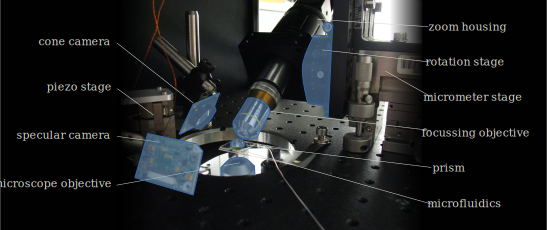
\includegraphics[keepaspectratio]{experimental/figures/spr_annotatedexperiment.pdf}
 \caption{Annotated picture of the experimental setup.  Description in the
	text.}
 \label{fig:experimentalpicture}
\end{figure}

An image of experimental setup for SPP experiments is shown in
\Figure{fig:experimentalpicture} with the important components annotated.
A simplified schematic of the same setup is also shown in
\Figure{fig:experimentalsetup}.

Light from a \SI{50}{\milli\watt} \SI{660}{\nano\meter} diode laser with a
bandwidth of \SI{30}{\giga\hertz} is first coupled into a single mode
optical fiber via an integrated air-spaced doublet fiber collimator.  The
fiber guides the laser light to an optical breadboard mounted on an
inverted microscope.  All primary functions of the experimental setup take
place on the breadboard.  Here, the Gaussian beam from the single mode
fiber is collimated by an output coupler to a beam waist of
$w_0=\SI{5}{\milli\meter}$ and proceeds through a polarizing beamsplitter,
passing $p$ polarized light.  The light is focused by a 10X microscope
objective onto the hypotenuse of a hemispherical prism of diameter
$d=\SI{10}{\milli\meter}$.  The beamsplitter and microscope objective are
mounted on a rotation stage which itself is mounted on a micrometer stage.
The objective itself is mounted on a zoom housing enabling linear travel
along the optical axis.  When the rotation stage is at the surface plasmon
resonance angle, the micrometer $z$ axis is fixed with a diffraction
limited spot at the center of the prism's hypotenuse.  The size of the spot
can then be modified via the zoom housing, and its transverse location on
the surface by the $x$ and $y$ lead screws on the micrometer stage.  
\begin{figure}[ht]
\centering
 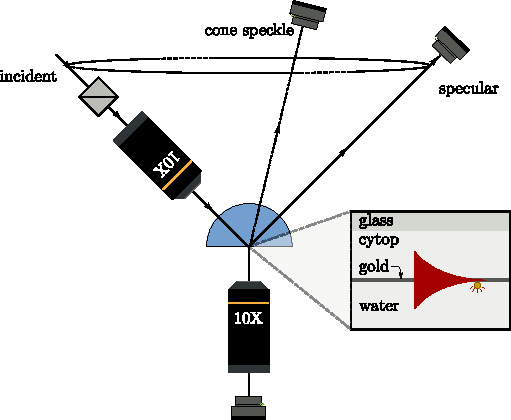
\includegraphics[keepaspectratio]{experimental/figures/conefig.pdf}
 \caption{Schematic of the experimental setup.  Description in text.}
 \label{fig:experimentalsetup}
\end{figure}

The hemispherical prism is mounted on a planar structure supporting either
normal or long range SPPs.  Reverse of this structure is a microfluidic
flow cell where samples can be introduced.  The specularly reflected and
scattered light containing information from SPP interference and scattering
is ultimately recorded at desired locations with a series of imaging
sensors.

Both the microfluidics and the substructure supporting the prism are thin
and optically transparent.  In this way, the sensing surface may be imaged
with an objective from the inverted microscope.  The breadboard containing
the experiment was fixed to the optical table with its own micrometer
stage, permitting translation of the entire experiment in the plane of the
optical table.

We experimented with several different focussing strategies in the
refinement of the experiment, and found that a microscope objective is the
simplest choice.  Because microscope objectives fulfil the sine condition,
focussing to the central point on the hypotenuse of a hemispherical prism
should introduce a minimum amount of aberrations.

Extra attention was not given to mechanical stability.  Though most of the
stages were high quality, the mounting of components such as the imaging
sensors and the prism on its glass slide were less than what would normally be considered optically rigid.
We did not observe any negative effects resulting from these choices.

\subsection{Imaging Sensor}
As stated, light from the experiment was directly recorded with imaging
sensors at select locations around the ring.  Because no optics besides the
hemispherical prism itself were used in this capture, we desire the sensors
to be close to the prism in order to capture the largest area of cone
features possible.  To facilitate this, the sensors were removed from their
housings and the naked PCB used as a mount support as in
\Figure{fig:imagingsensor}.
\begin{figure}[ht]
 \centering
 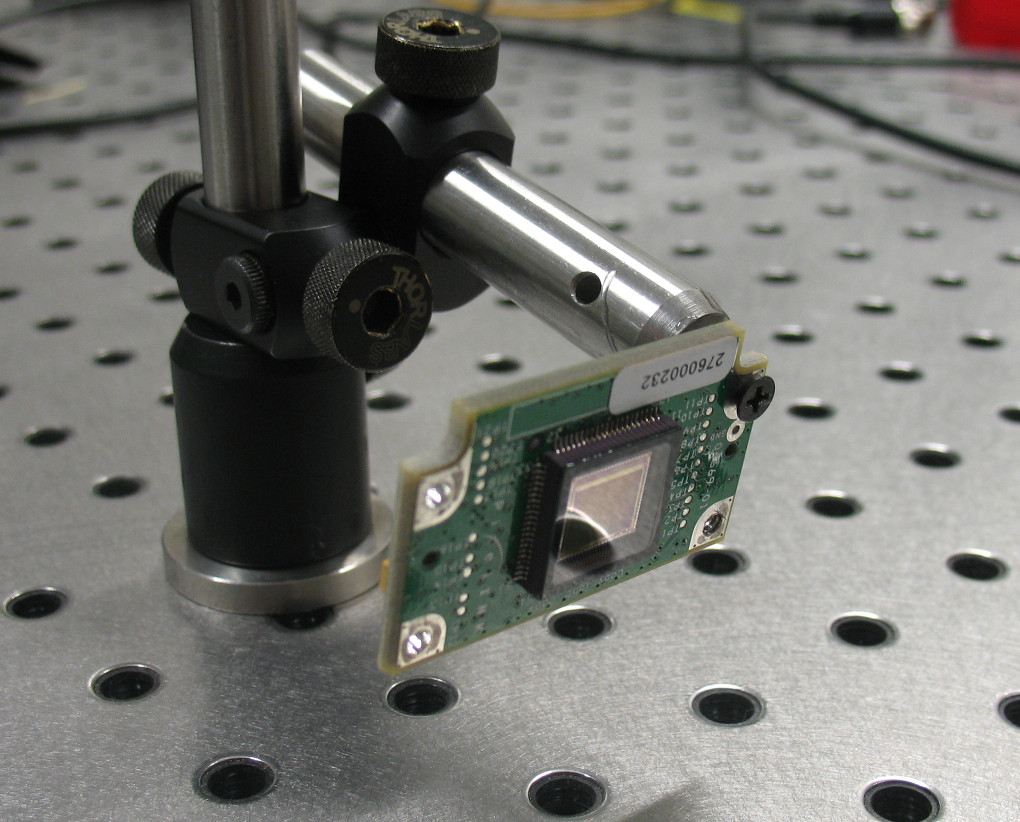
\includegraphics[width=6cm,keepaspectratio]{experimental/figures/nakedsensorcrop.jpg}
 \caption{Imaging sensor removed from its housing.}
 \label{fig:imagingsensor}
\end{figure}

Two types of imaging sensors were used in the experiment: an IDS USB 2.0
\SI{8}{\bit} CMOS camera and a PixelGrey IEEE-1394 (Firewire) \SI{16}{\bit}
CCD.  Both had a spatial resolution of $1280\times1024$ pixels.  The
cameras are capable of what is known as a ``limited area of interest''
(AOI).  This feature allows the cameras to capture a subset of their
available pixel region before the information traverses the serial bus to
the host computer.  The IDS datasheet specifies that in AOI mode, with
sufficient lighting conditions framerates of up to \SI{250}{fps} are
possible.  We have found that this framerate was a limitation imposed due
to bad design of both the stock acquisition software and the USB serial
bus, and with simple modifications this can be extended to over
\SI{1400}{fps} for the smallest AOI.

The modifications were carried out in the following way.  On the software
side, we used the IDS UEye SDK version 3.82 to read the raw sensor data
directly from camera memory and write it to a single binary file on the
disk of the host computer.  This has two speed advantages compared with the
default method.  First, it suppresses all calls to image or video libraries
by removing the need to transcode the pixel data.  Second, saving to a
single file is much faster than saving to multiple files because it
elliminates seeking of the computer's physical disk read/write head during
both file creation and updating the disk's filesystem journal.  

On the hardware side, we found it necessary to assign each USB camera to
its own dedicated USB bus.  This allowed us to maximize the USB polling
frequency and avoid traffic on the bus which would otherwise interrupt the
datastream.  Firewire cameras did not need this effort, as the IEEE-1394
protocol supports isochronous transfers which are able to guarantee a
device a certain amount of bandwidth.

%(480 megabits per second)/((1280*128*8 bits) per frame)
